\section{Implementation}
\label{sec:implementation}

% \begin{itemize}
%   \item Extension of the library RxLua
%   \item Why reactive?
%     \url{http://www.reactivemanifesto.org/}
%   \item ØMQ Lua bindings
%   \item ØMQ queues with push/pull protocol - Fire-and-forget messaging: a messsaging pattern in which we do not expect a direct response to the message, as opposed to request-response protocols
% \end{itemize}

%On September 2014 has been published the Reactive Manifesto\cite{reactivemanifesto}.
%This one attempts to define the principles to build systems more flexible, loosely-coupled and scalable.
%A \textit{reactive system} has to follow the four Reactive Principles:
%
%\begin{itemize}
%  \item Responsive: it is quick to react to all users in order to ensure a consistently positive user experience;
%  \item Elastic: it is easily upgraded on demand in order to ensure responsiveness under various load conditions;
%  \item Resilient: it applies proper design and architecture principles in order to ensure responsiveness;
%  \item Message-driven: it is based on a message-passing architecture to establish a boundary between components that ensures loose coupling, isolation and location transparency, e.g. event-driven, actor-based, or both of them.
%\end{itemize}
%
%The responsiveness of a system needs both elasticity and resiliency.
%Finally, a message-driven architecture is the foundation of elastic, resilient and responsive systems, as shown on figure \ref{fig:reactive-traits}.
%
%\begin{figure}[t!]
%  \centering
%  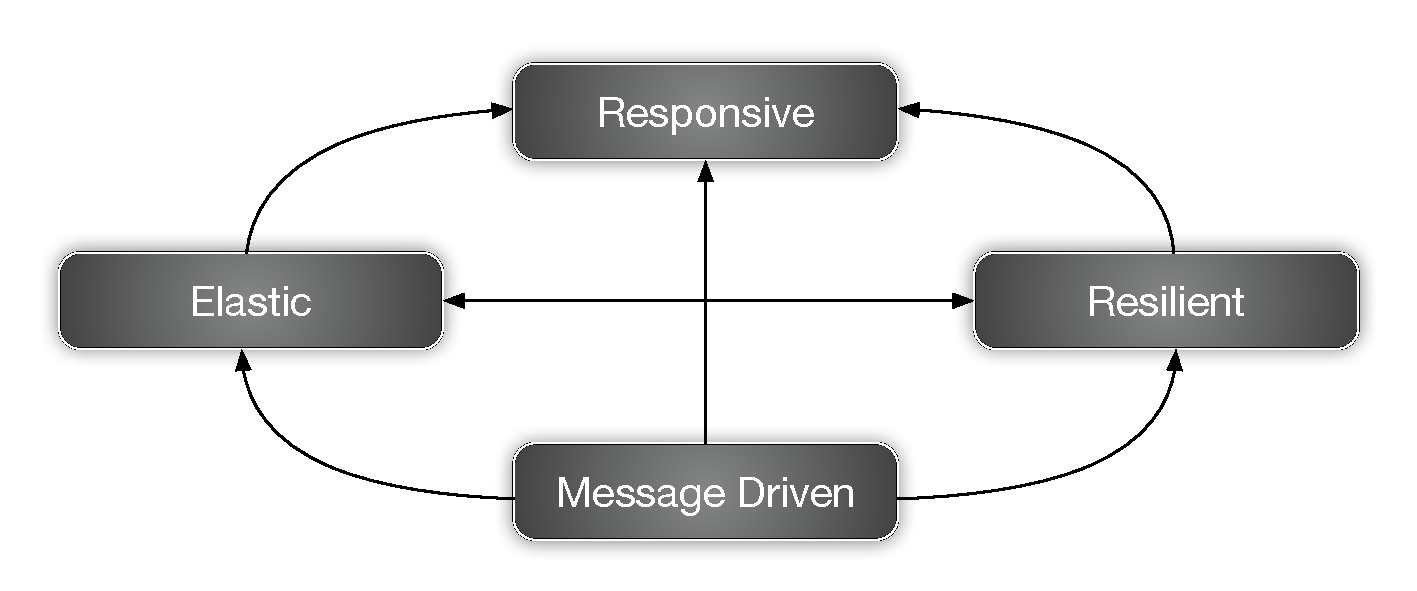
\includegraphics[width=.99\linewidth]{images/reactive-traits}
%  \caption{Reactive traits.}
%  \label{fig:reactive-traits}
%\end{figure}
%
%
%The term \textit{reactive} is not new in the field of computer sciences: Gérard Berry used it in 1989 while talking about \textit{real-time programming}\cite{berry:realtime_programming}.
%But recently the industry recognized the \textit{reactive paradigm} as the de facto way forward in system design\cite{malawski:why_reactive}.
%In the field of data streams, \textit{reactive programming} is programming with asynchronous streams, anything else.
%A stream is a sequence of ongoing events ordered in time, and these emitted events are captured only asynchronously by defining three functions:
%
%\begin{itemize}
%  \item an \textbf{onNext} function that will execute when a value is emitted;
%  \item an \textbf{onError} function executed when an error is emitted;
%  \item and finally an \textbf{onComplete} function executed when the stream is over.
%\end{itemize}
%
%
%
%A plenty of software libraries for different languages ensues from this paradigm\cite{reactive_streams}\cite{github:reactive_streams}.
%As exposed in section \ref{sec:architecture}, we chose the Lua technology as the basic of \SYS's implementation.
%Lua is a scripting language that is simple, efficient, extensible, functionnal and open-source\cite{ierusalimschy_programming_2006}.
%It will be easy to handle for the end user of \SYS.
%By the way, it is embedded in many application programs, such as Adobe Lighroom, Nmap, World of Warcraft or Nginx.


\SYS is implemented in Lua (v5.3).
Our implementation is compact, as it consists of only 120 lines of code (without counting the dependencies).
The framework partially extends \rxl~\cite{github:rxlua}, a library for reactive programming in Lua.
\rxl provides to the developer the required API to design a data stream processing pipeline following a dataflow programming pattern~\cite{uustalu_essence_2005}.
Listing~\ref{pipeline-example} shows an example of a \rxl program (and consequently, a \SYS{} program) to compute the average age of a population by chaining \texttt{:map}, \texttt{:filter} and \texttt{:reduce} functions.
The \texttt{:subscribe} function performs the subscription of 3 functions to the data stream.
These functions are observers, and the stream is an observable: this is precisely an implementation of the \textit{Observer Design Pattern}~\cite{szallies_using_1997}.
%A simple program example, computing from a source of \textit{people} the average age of the adult ones, throw a map/filter/reduce pipeline, is presented in listing \ref{pipeline-example}.

\SYS{} dynamically ships the business logic for each component into a dedicated Docker container and executes it.
%Our extension takes the business logic in each element of the pipeline to send and execute it in a Docker container.
The communication between the Docker container happens through \zmq (v4.1.2) and the corresponding Lua bindings~\cite{github:lzmq}.
%Then, the data is streamed accross the network communication built on top of the ØMQ protocol and implemented using the ØMQ Lua bindings\cite{github:lzmq}.
In summary, \SYS{} abstracts the underlying infrastructure from the developer, relying on \zmq and Docker.
We plan to release our code as open-source.

\begin{minipage}{\linewidth}
\begin{lstlisting}[language=LUA,caption={Process pipeline example, using the library RxLua},label=pipeline-example]
Rx.Observable.fromTable(people)
 :map(
   function(person)
     return person.age
   end
 )
 :filter(
   function(age)
     return age > 18
   end
 )
 :reduce(
   function(accumulator, age)
     accumulator[count] = (accumulator.count
       or 0) + 1
     accumulator[sum] = (accumulator.sum
       or 0) + age
     return accumulator
   end, {}
 )
 :subscribe(
   function(datas)
     print("Adult people average:",
       datas.sum / datas.count)
   end,
   function(err)
     print(err)
   end,
   function()
     print("Process complete!")
   end
 )
\end{lstlisting}
\end{minipage}
